Continuing in our goal of illustrating how algebraic effects enable programmers to deal with the interaction of variation and side effects, we show the rest of the file I/O library in reading. Reading is more complex than writing because we need to manage different vitiation contexts of the same file (simulate multiple plain files at once). To illustrate how reading should work, follow the sequence of operations in Figure \ref{fig:file-figures}. 

%
\begin{figure}[!htb]
\begin{subfigure}[b]{.33\textwidth}
  \centering
  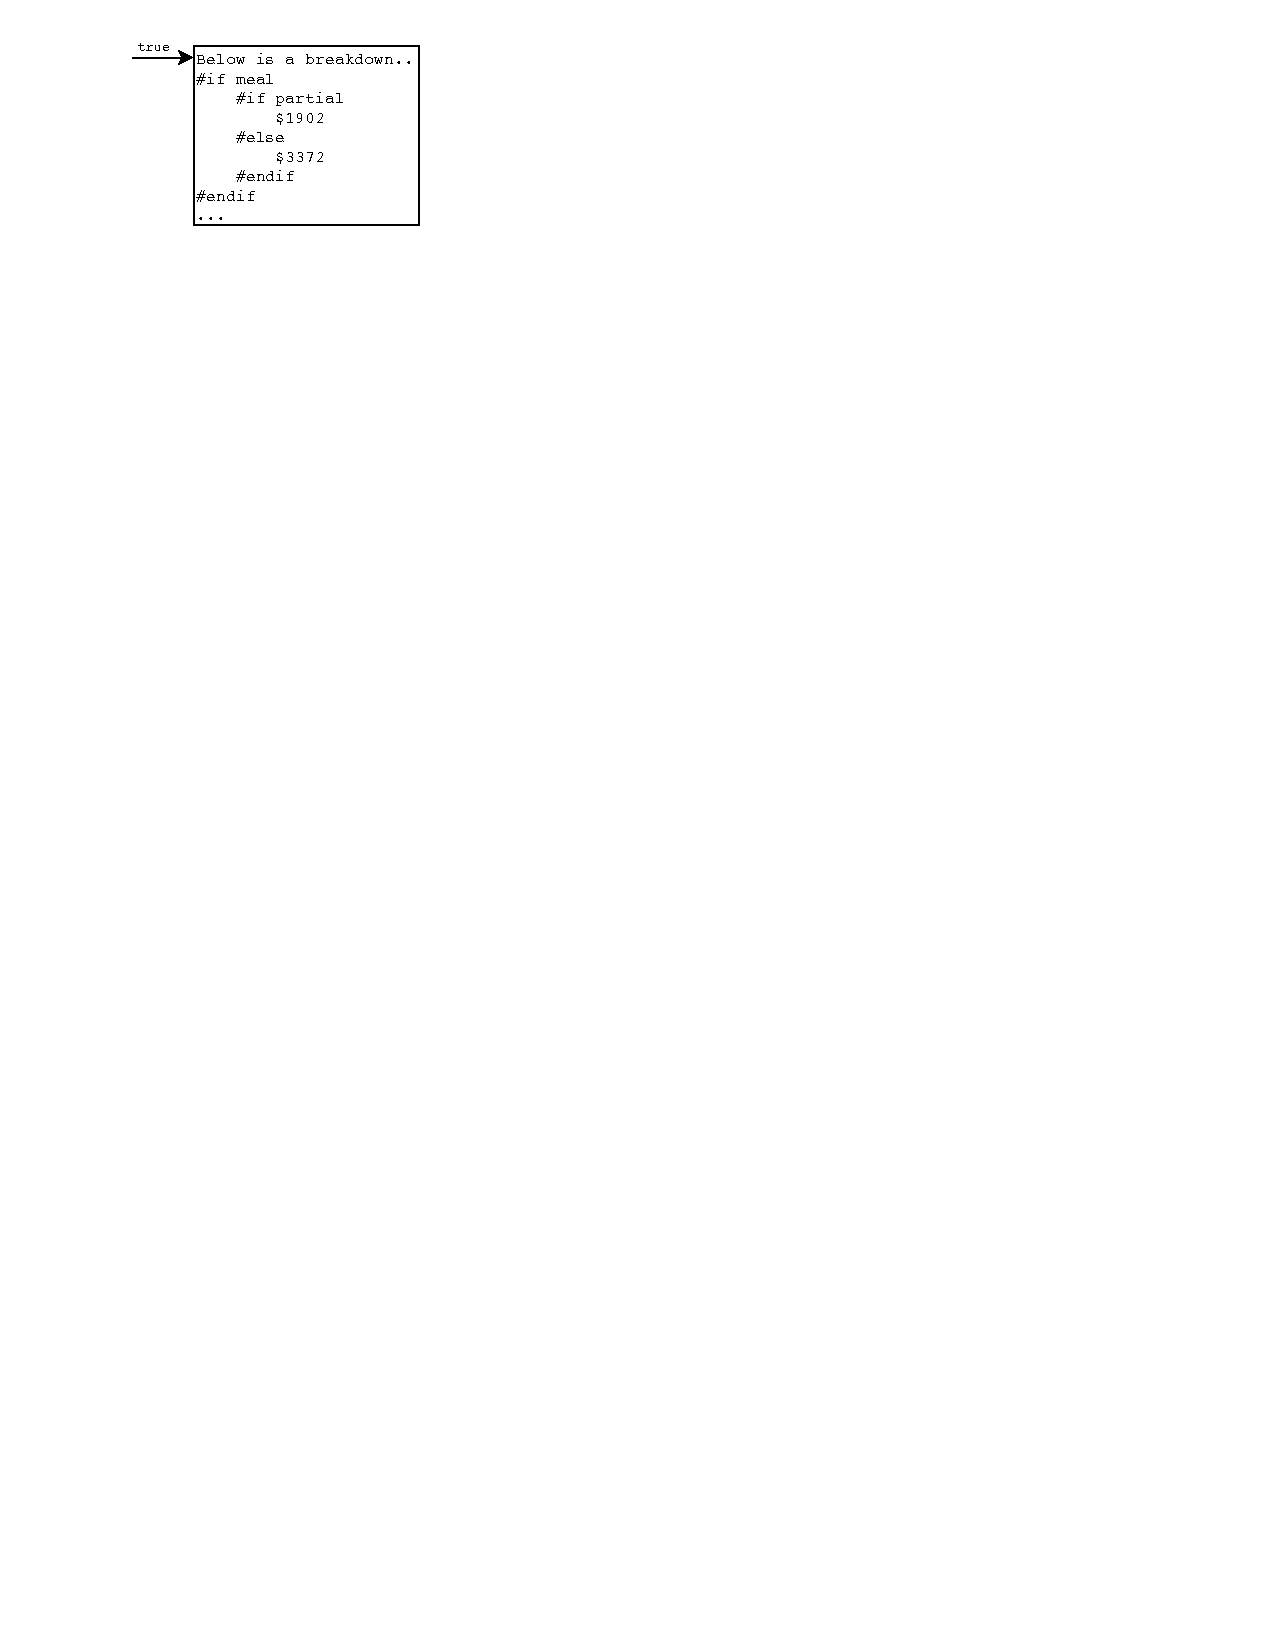
\includegraphics[scale=0.75]{figures/vfile-Page-1.pdf}
  \caption{Read-line in context \texttt{true}.}
  \label{fig:file1}
\end{subfigure}
\begin{subfigure}[b]{.33\textwidth}
  \centering
  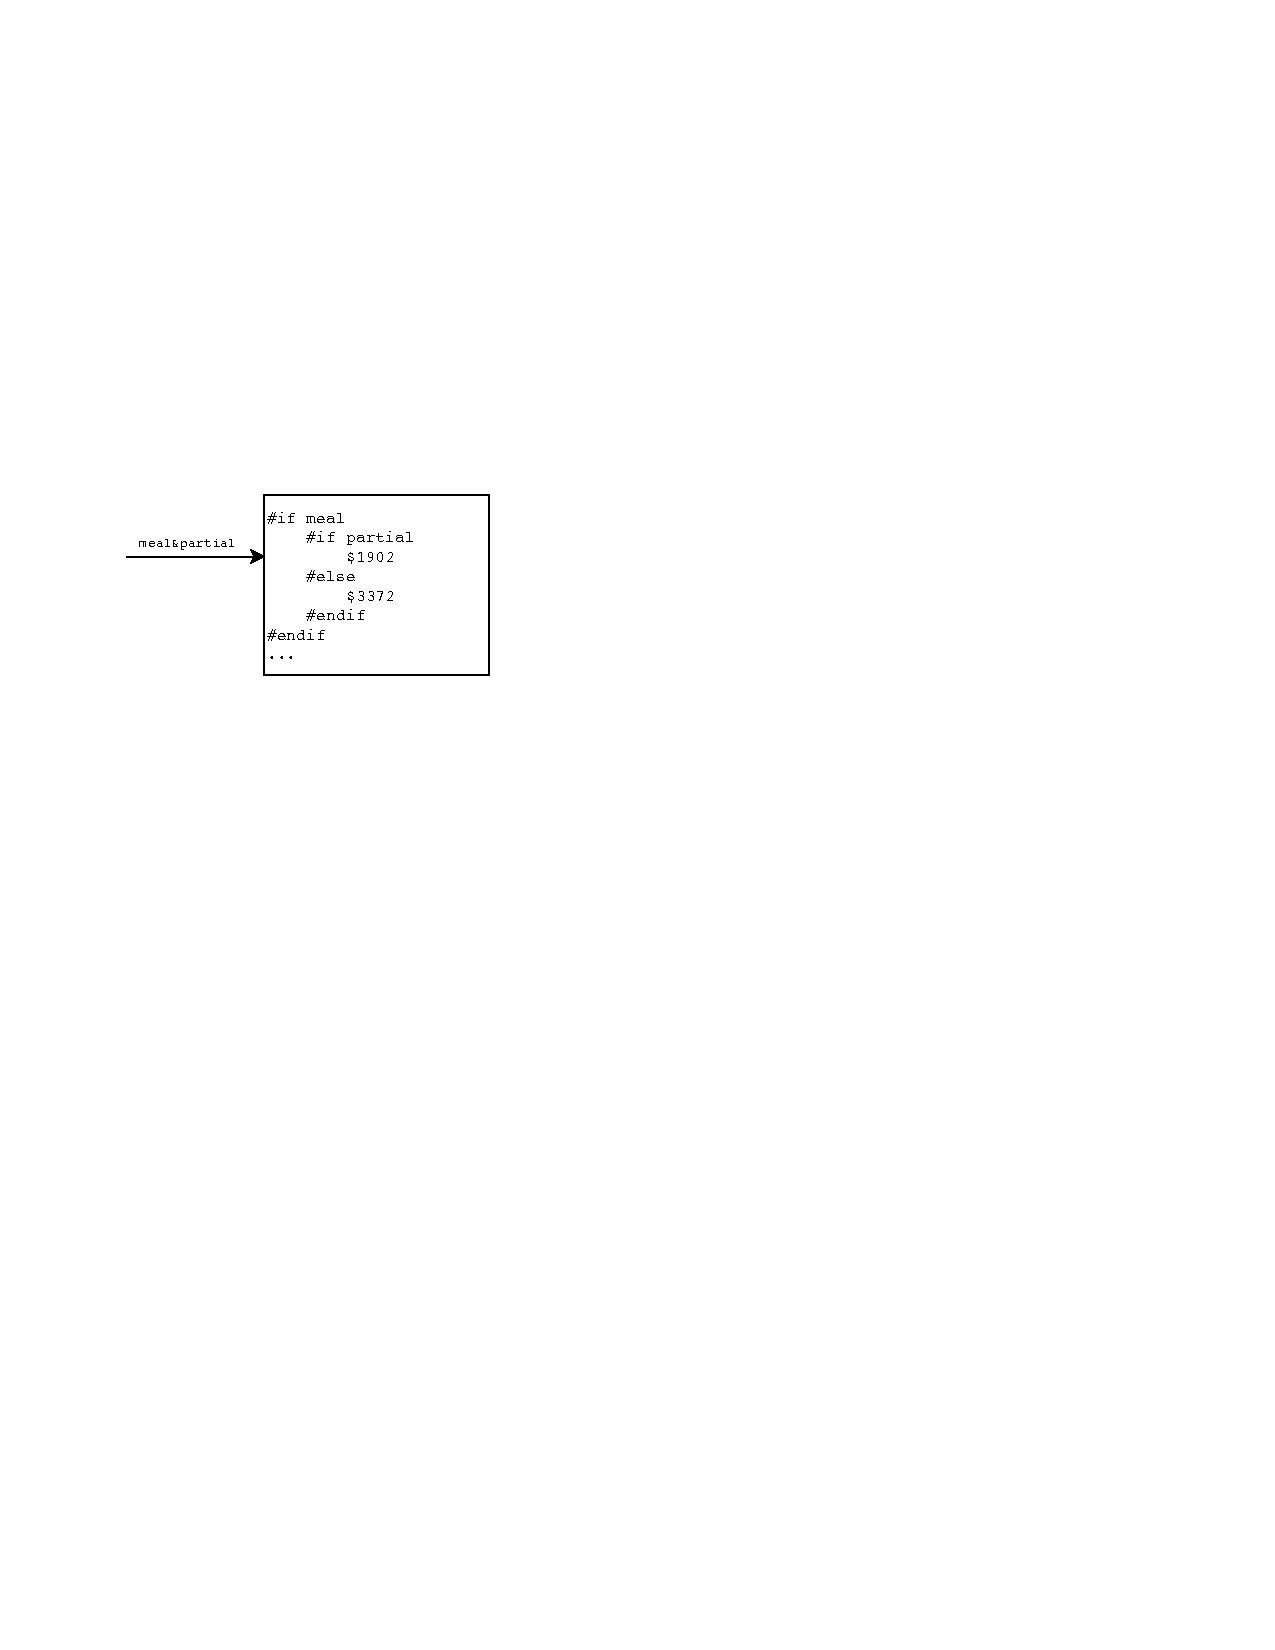
\includegraphics[scale=0.75]{figures/vfile-Page-2.pdf}
  \caption{Read-line in \texttt{meal\&partial}.}
  \label{fig:file2}
\end{subfigure}
\begin{subfigure}[b]{.33\textwidth}
\centering
  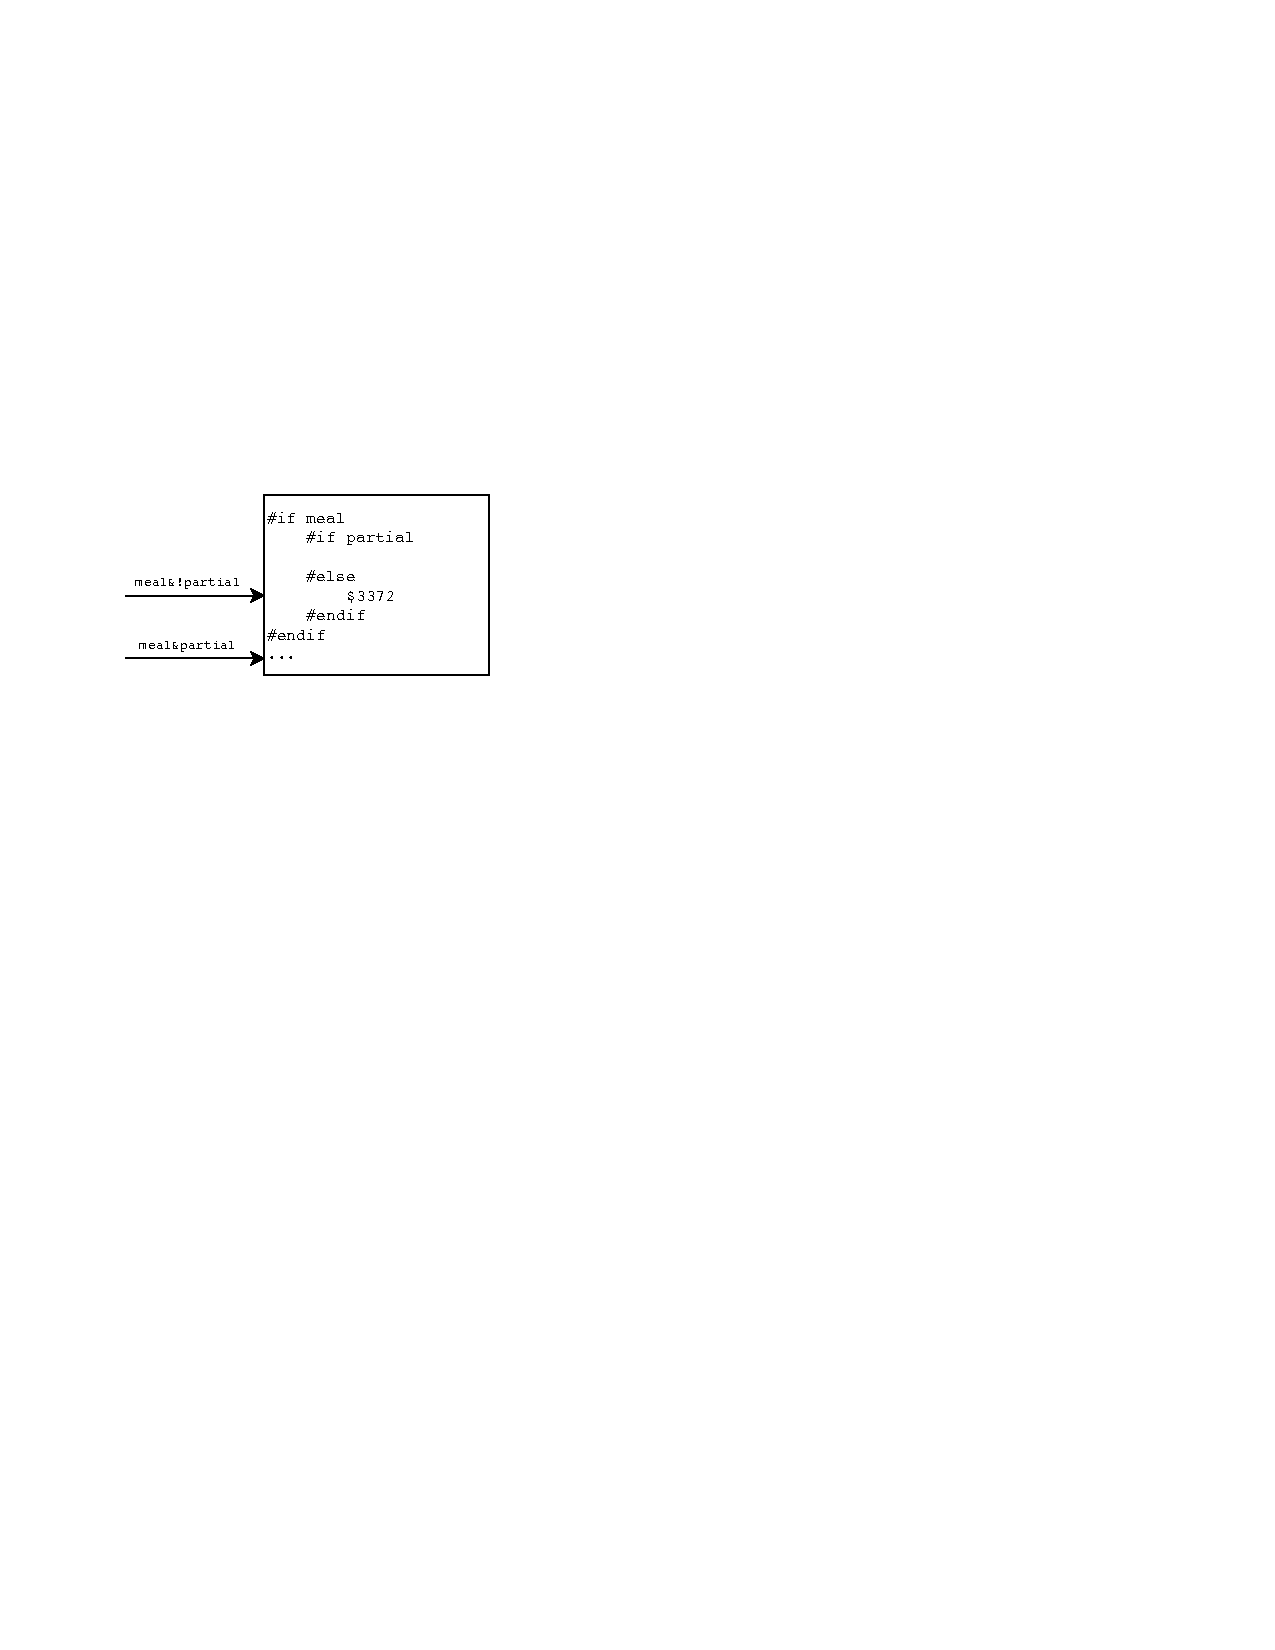
\includegraphics[scale=0.75]{figures/vfile-Page-3.pdf}
  \caption{Read-line in \texttt{meal\&!partial}.}
  \label{fig:file3}
\end{subfigure}
  \caption{File representation in a sequence of read-line operations.}
  \label{fig:file-figures}
\end{figure}
%

Plain read-line calls have context \texttt{true} by default. When we start to read from the file, the file pointer is at the first line of the file with context \texttt{true} as shown in Figure \ref{fig:file1}. We perform a read-line operation as shown below.
%
\begin{lstlisting}[escapeinside={(*}{*)}]
readLine file = "Below is a breakdown.." 
\end{lstlisting}
%
Reading in context \texttt{true} corresponds to reading from all file variants. Since the first line is plain, it is available in all variants, so we return it. 

We then perform a second read-line operation in the context \texttt{meal\&partial} as shown below.
%
\begin{lstlisting}[escapeinside={(*}{*)}]
(*$\Opt[\texttt{(meal\&partial)}]{\texttt{readLine file}}$*) = "$1902"
\end{lstlisting}
%
The file pointer now moves to the true alternative of the choice \texttt{partial} in line 2 as shown in Figure \ref{fig:file2} and we return the line \texttt{"\$1902"} corresponding to this context. 
%

We then perform a third read-line operation but in the context \texttt{meal\&!partial} as shown below.
%
\begin{lstlisting}[escapeinside={(*}{*)}]
(*$\Opt[\texttt{(meal\&!partial)}]{\texttt{readLine file}}$*) = "$3372"
\end{lstlisting}
%
We end up with two file pointers at two different locations. One with the context \texttt{meal\&!partial} pointing to the false alternative of the choice \texttt{partial} in line 2 and the other with context \texttt{meal\&partial} pointing to the third line as shown in Figure \ref{fig:file3}. We return the line \texttt{"\$3372"} corresponding to the context \texttt{meal\&!partial}. 

In the rest of this section, we show how we could manage these variational read-line calls and how we extend the environment to support file reading using algebraic effects. 

\section{Variational Queues for Representing Files}
\label{sec:queue_to_file}

We need to use a special data structure that could simulate the different plain files corresponding to different variation contexts in a variational file. Therefore, we use the variational queue implementation in Chapter \ref{sec:queue_lib} to represent files. This way we could load variational lines from the file into the queue using enqueue operations and read-lines from the file through dequeue operations. However, we still need to parse lines from the variational text file to be able to enqueue them.

In this section we show how to parse variational files into variational queues. The parser details are shown in Figure \ref{fig:parser}. The parser takes a variational text file as input and returns a variational queue as output. The queue is initialize to empty at the beginning. Parsing mainly occurs in the helper function \texttt{read}. The function \texttt{read} takes a file channel, queue, text and context as parameters. The text corresponds to the last line of text read from the file. The queue is updated with enqueue operations after parsing each line (plain or variational). The context corresponds to the context of a parent variational line if it exists; it is \texttt{true} by default.

%
\begin{figure}[h]
 \begin{lstlisting}
let rec read file q text ctx =

    if is_choice text then
        let ctx' = get_ctx text in 
        read_vline file q ctx ctx'
    else  
        enqueue' q text (Lit true)
        
and read_insert file q line ctx ctx'= 

    if is_choice line then 
        read file q line ctx'
    else 
        enqueue' q line (And (ctx',ctx)) 
				 
and read_vline file q ctx ctx' = 

    let line = get_next_line file in 
	
    if is_endif line then 
        q
    else if is_else line then 
        read_vline file q ctx (Not ctx')
    else
        let q' = read_insert file q line ctx ctx' in
        read_vline file q' ctx ctx'
;;
\end{lstlisting}
  \caption{Variational file parser.}
  \label{fig:parser}
\end{figure}

In the function \texttt{read}, we check if the text corresponds to a variational line by checking if it starts with the keyword \texttt{\#if}. If the text corresponds to a plain line, we directly enqueue it with context \texttt{true}. Otherwise, we parse the variational line in the helper function \texttt{read\_vline}. We pass two contexts as parameters: the context of the underlying choice (\texttt{ctx'}) and the context of any parent line (\texttt{ctx}).

In the helper function \texttt{read\_vline}, we read a line from the file, then determine in which variant of the variational line we are. If the line has the keyword \texttt{\#end}, we return the queue unchanged. If the line has the keyword \texttt{\#else}, we recursively invoke \texttt{read\_vline} with the negation of the context corresponding to the underlying choice (\texttt{ctx'}). Otherwise, we invoke the function \texttt{read\_insert}, which would insert the text of the underlying variant into the file. Then, we recursively invoke \texttt{read\_vline} again with the same context \texttt{ctx'} to parse the rest of the line. 

In the helper function \texttt{read\_insert}, we check if the variant has a nested variational line (choice). If there is a nested variational line, we recursively invoke \texttt{read} on it. Otherwise, we directly enqueue the line with its corresponding enqueue context. The corresponding enqueue context is the conjunction two context: the context of the parent variational line and the context of the underlying variational line. 


Besides parsing variational and plain lines, we also parse the contexts of variational lines. We show this parser code in the Appendix (Section \ref{sec:ctx_parser}).


\section{Variational Read-line}
\label{sec:file_read}

In this section, we write a new handler for the variation effect to support file reading and show an example of its use. We also show some useful applications of this work.

The handler \texttt{read\_v\_handler} in Figure \ref{fig:read-lib} allows us to perform read-line operations in variation. It also has a similar behavior to the variation handler in Figure \ref{fig:choice-impl} for handling the choice operations. However, in this handler we run the alternatives of the choice and return their corresponding results. In addition, we mange the variation context (or context for short), which helps separate the effects of the choice alternatives. With this implementation, we are able to determine in which alternative of the choice we are and thus figure out its corresponding context. The context is by default \texttt{true} with plain read-line operations. Otherwise, we use the operations \texttt{if\_}, \texttt{else\_}, and \texttt{end\_} to mange it.

\begin{figure}
\begin{subfigure}[b]{.5\textwidth}
  \centering
 \begin{lstlisting}[]
let if_ d =
    let (s,l) = #Get() in 
    let l' = (d :: l) in
    #Set((conjList l',l'))  
;;    

 let end_ () = 
    let (s,l) = #Get() in 
    match l with
        [] -> #Set((conjList l, l))
        | (x::l') -> #Set((conjList l', l'))  
;; 

\end{lstlisting}
\end{subfigure} \hspace{1em}
\begin{subfigure}[b]{.5\textwidth}
  \centering
 \begin{lstlisting}[]
let else_ () =
    let (s,l) = #Get() in 
    match l with
        [] -> #Set((conjList l,l))
        | (s':: l') -> 
            let s'' = (Not s') in 
            let l'' = (s''::l') in
            #Set((conjList l'', l'')) 
;;
  		
\end{lstlisting}
\end{subfigure}
  \caption{Operations for managing the variation context.}
  \label{fig:c-form-impl}
\end{figure}


\begin{figure}[!h]
 \begin{lstlisting}[]
let read_line f ctx = dequeue ctx f;;

let read_v_handler = handler
    | #Choice s k ->
        if_ s;
        let l = (k true) in
        else_ ();
        let r = (k false) in
        end_ ();
        (Chc (s,l,r))
    | #Read_line _ k -> k "c"
    | val x -> 
        if (is_empty x) then 
            Hole
        else 
            let q = #GetQueue() in
            let (c,_) = #Get() in
            let (r,q') = read_line q c in
            #SetQueue(q');  
            r
;;

let readLine () = #Read_line dfile;;

let read_line_h f = 
    with read_var_line_handler handle
        f ()
;;

let opt d t = chc d t "";;
\end{lstlisting}
\caption{File reading library.}
\label{fig:read-lib}
\end{figure}

The variation context is implemented as a mutable state (the algebraic effect and handler definitions for state are discussed in Section \ref{sec:background}) that holds a stack of contexts. To make things easier, we also hold the current context in the state making a tuple of two arguments: the current context and the stack of contexts. The entire implementation is shown in Figure \ref{fig:c-form-impl}. The first operation \texttt{if\_} takes a boolean formula over options and pushes it into the stack of contexts. The second operation \texttt{else\_} pops the top element (a context) of the stack and pushes the negation of it into the stack. The third operation \texttt{end\_} pops the top element (a context) of the stack. In every case after updating the stack of contexts, we update the current context to be the conjunction of all contexts in the stack.

Besides the variation context, we also manage another state in this handler which holds the variational queue representing the file. We choose to hold it in the state to avoid passing it between read-line operations. 

For catching the built-in effect operation \texttt{\#Read\_line}, which has a return type of string, we simply keep the continuation running with a default string. Note that we can neglect passing the file in every call to \texttt{\#Read\_line} and use a default file instead because the corresponding file representation is already passed to the handler. 

In the return case, we retrieve from the states both the variation context and the variational queue (representing the file). Then, we perform the \texttt{read\_line} operation on the file with the given variation context. The operation \texttt{read\_line} is basically a dequeue operation on the variational queue, which takes the variation context as parameter. The result of performing dequeue is a tuple of two arguments: the resulted line and the updated variational queue. The state holding the queue is set to the new queue \texttt{q'} and the result \texttt{r} is returned. Note that the return value of \texttt{read\_line} has type \texttt{v} because the result is either a plain line of text (\texttt{One}), a variational line (\texttt{Chc}), or nothing (\texttt{Hole}). 

Using this mechanism, we could read lines from variational or plain files, as shown below. 
%
\begin{lstlisting}[escapeinside={(*}{*)}]
let r_file = #Open_in "file.eff" ;;
let queue = read_v r_file;;
#Close_in r_file;;

let line1 () = readLine () ;;
let line2 () = (*$ \Opt[\texttt{(meal\&partial)}]{\texttt{readLine () }} $*);;
let line3 () = (*$ \Opt[\texttt{(meal\&!partial)}]{\texttt{readLine ()}} $*);;

let f () =
	read_line_h line1 ; read_line_h line2 ; read_line_h line3
;;

read_lines_h queue f;;
\end{lstlisting}
%
We open the file and then load it in a variational queue using the operation \texttt{read\_v} which is a parser explain in Section \ref{sec:queue_to_file}. After that, the file could be closed because the queue would be used instead to represent the file. The helper function \texttt{read\_line\_h} is used to wrap syntax of the variational read handler. The operation \texttt{read\_lines\_h} is used to wrap the syntax of states' handlers (variational queue state and variation context state). The example above shows the same sequence of read-line operations in Figure \ref{fig:file-figures}.

Because the results from read-line could be variational, we combine our work in file reading and variation to concatenate lines. 
%
\begin{lstlisting}[escapeinside={(*}{*)}]
let line1 () = readLine ();;
let line2 () = (*$ \Opt[\texttt{meal}]{\texttt{readLine ()}} $*);;

let g () =
    let res1 = read_line_h line1 in 
    let res1 = read_line_h line2 in 
    let r () = 
        let a1 = reflect_v res1 in
        let a2 = reflect_v res1 in
        a1 ^ "  " ^ a2 
    in reify_v r 
;;

read_lines queue g;;
\end{lstlisting}
%
We use the \term{reify} and \term{reflect} technique, which are the inverse of each other, to accomplish that. In reflect, we convert the \texttt{v} type result into a choice effect operation and in reify, we calculate the corresponding variational result using the variation handler in Figure \ref{fig:choice-impl}. The example above concatenates the results of two read-line operations. The first is a plain read-line operation and the second is a variational read-line operation with the context \texttt{meal}.
The result \texttt{a1} is a plain line of text while the result \texttt{a2} is a choice as shown below.  
%
\begin{lstlisting}[escapeinside={(*}{*)}, backgroundcolor = \color{lightgray}]
a1 = (*\texttt{"Below is a breakdown of the preliminary housing costs for 2018-2019."} *)
a2 = (*\Chc[\texttt{partial}] {\texttt{"\$1902"} }{\text{"\$3372"}} *) 
\end{lstlisting}
%
Therefore, the final result of concatenating the lines above is the following variational value.
%
\begin{lstlisting}[escapeinside={(*}{*)}, backgroundcolor = \color{lightgray}]
(*\Chc[\texttt{partial}] {\texttt{"Below is a breakdown of ..  \$1902"}}{\texttt{"Below is a breakdown of ..  \$3372"}} *)
\end{lstlisting}
%
This implementation enables us to see the results corresponding to different variants in one run of the program. 

The next example is another useful application that shows how the integration of variation and side effects can prevent from repetitive work. Being able to read all alternatives of the file at once, allows performing a filter operation on all alternatives at one run and getting the variational value of all alternatives. The following program counts the number of times the text "\$13360" occurs in any alternative of the variational file. 
%
\begin{lstlisting}[]
let checkDocs w q =
  let words = concatMap (fun str -> split str x) q in
  let matches = filter (fun a -> a = w) words in
  length matches
;;
			
let q' () = map (fun v -> (reflect_v v)) q in
let f ()  = checkDocs "$13360" (q' ()) in
reify_v f ;;

\end{lstlisting}

In a similar manner, we run a map operation converting every line to a choice operation (reflect). Then, we calculate the variational result using the variation handler (reify). In each alternative, we run the filter operation \texttt{checkDocs}. Running this program on the example file in Figure \ref{fig:file_example} will result \texttt{2} when the two expressions (\texttt{artists' residence \& (single | efficiency)}) and (\texttt{smith \& (!kitchen \& single)}) are true, \texttt{1} when only one of them is true, and \texttt{0} when both are false. The following choice represents the result (we use artists instead of artists' residence for short).
%
\begin{lstlisting}[numbersep=6pt, escapeinside={(*}{*)}, backgroundcolor = \color{lightgray}]
(*\Chc[\texttt{(artists\&(single|efficiency))}]{\Chc[\texttt{(smith\&!kitchen\&single)}]{2}{1}}{\Chc[\texttt{(smith\&!kitchen\&single)}]{1}{0}} *)
\end{lstlisting}




% In \texttt{read}, if the line was a plain text, it is inserted into the stack with the context \texttt{true} (line 25). If the line was variational (choice), the parser runs the algorithm below (line 22-23). The algorithm is almost identical for the left and right alternatives of the choice and shown in the helper function \texttt{read\_vline}. To indicate in which alternative we are, we pass the variable \texttt{fileCtx} which is either \texttt{L} or \texttt{R}. We start running this algorithm in the left alternative (\texttt{L}). 

% \begin{enumerate}

% \item (Line 4): to avoid getting into the end of file (eof), \texttt{get\_maybe\_next\_line} checks the maybe type line that was passed to the function. If the line has been read already, the line is wrapped in a \texttt{Just} constructor. Otherwise, \texttt{Nothing} is passed, which indicates that we should read the next line from the file. 

% \item (Lines 5-6): we first check if the line has the keyword \texttt{\#end} which happens in the case where there is an empty string in the else branch. If so, we return an empty list. Otherwise, we do the next steps. 

% \item (Lines 8-12): to find the next line to be returned (\texttt{next\_return\_line}), we check whether or not the line we are processing is a sub-choice. If it is so, we have to recursively call \texttt{read} to parse the sub-choice. Otherwise, we return the plain line from step 1. 

% \item (Line 12): the context of the line we return differs based on the value of \texttt{fileCtx} (\texttt{L} | \texttt{R}). If we are in the left alternative (\texttt{L}), the context stays the same. If we are in the right alternative (\texttt{R}), the context is negated. This is done int the function \texttt{upd\_ctx}.

% \item (Line 10): for sub-choices, the context is the conjunction of the updated context in the previous step and the context of the parent choice. This is done int the function \texttt{calc\_ctx}. 

% \item (Lines 15-20): after figuring out the next return line, we check if there is a keyword next, which guides to the next step. 
% \begin{itemize}

% \item (Lines 15-16): If we found the keyword \texttt{end}, we return the next return line from step 3.
% \item (Lines 17-18): if we found the keyword \texttt{else}, we repeat the algorithm but with the \texttt{fileCtx} (\texttt{R}) parsing the right alternative of the choice. We concatenate that with next return line from step 3.
% \item (Lines 19-20): if we found no keyword, we repeat the algorithm in the same alternative because having no keywords indicates that there are more lines of text in the same alternative. We concatenate that with next return line from step 3.
% \end{itemize}

% \end{enumerate}